\hypertarget{ux446ux435ux43bux44c-ux440ux430ux431ux43eux442ux44b}{%
\chapter{Цель
работы}\label{ux446ux435ux43bux44c-ux440ux430ux431ux43eux442ux44b}}

Изучить основы программирования в оболочке OC UNIX. НАучиться писать
небольшие командные файлы.

\hypertarget{ux432ux44bux43fux43eux43bux43dux435ux43dux438ux435-ux43bux430ux431ux43eux440ux430ux442ux43eux440ux43dux43eux439-ux440ux430ux431ux43eux442ux44b}{%
\chapter{Выполнение лабораторной
работы}\label{ux432ux44bux43fux43eux43bux43dux435ux43dux438ux435-ux43bux430ux431ux43eux440ux430ux442ux43eux440ux43dux43eux439-ux440ux430ux431ux43eux442ux44b}}

\begin{enumerate}
\def\labelenumi{\arabic{enumi}.}
\tightlist
\item
  Пишем скрипт, который архивирует сам себя и перемещает в директорию
  backup в домашнем каталоге
\end{enumerate}

\begin{figure}
\hypertarget{fig:001}{%
\centering
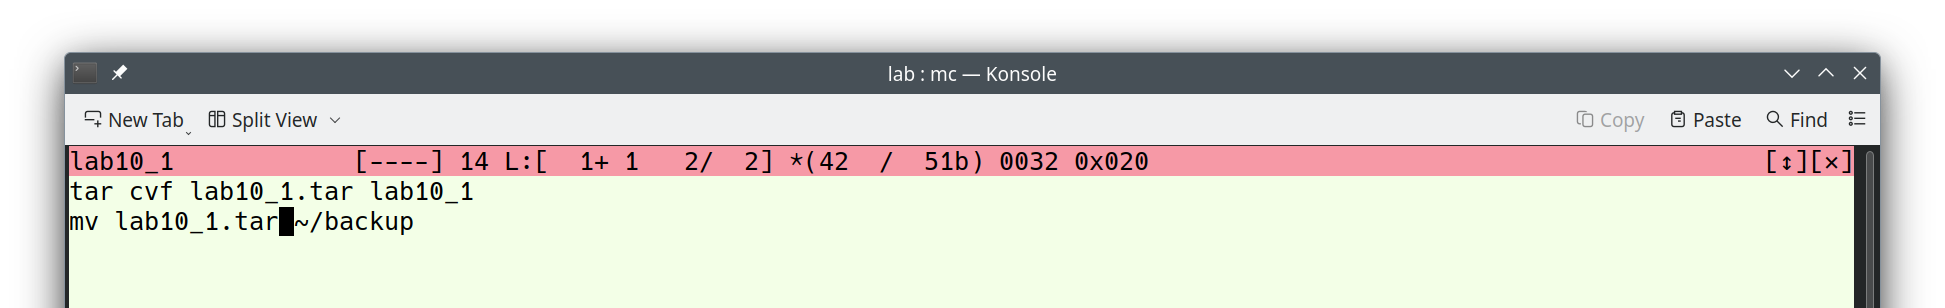
\includegraphics[width=1\textwidth,height=\textheight]{image/1.png}
\caption{код}\label{fig:001}
}
\end{figure}

\begin{figure}
\hypertarget{fig:002}{%
\centering
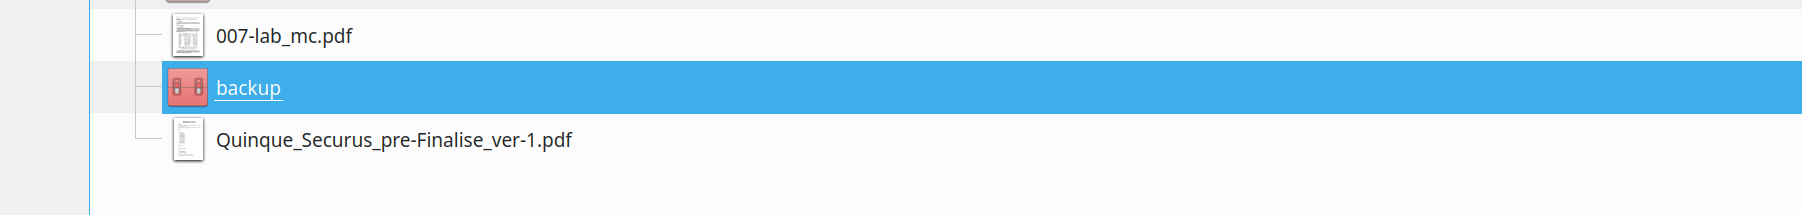
\includegraphics[width=1\textwidth,height=\textheight]{image/2.png}
\caption{backup в домашнем каталоге}\label{fig:002}
}
\end{figure}

\begin{figure}
\hypertarget{fig:003}{%
\centering
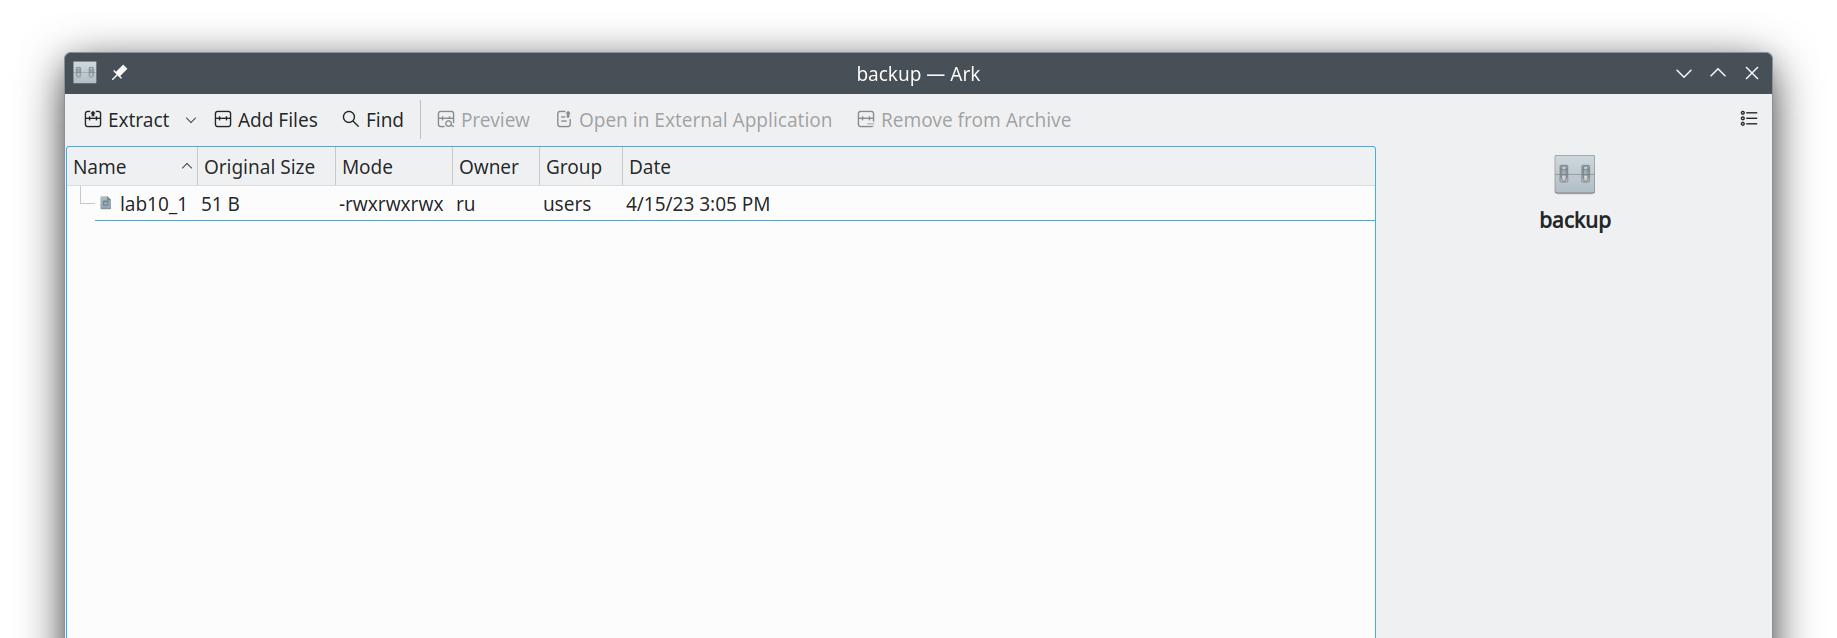
\includegraphics[width=1\textwidth,height=\textheight]{image/3.png}
\caption{содержание backup}\label{fig:003}
}
\end{figure}

\begin{enumerate}
\def\labelenumi{\arabic{enumi}.}
\setcounter{enumi}{1}
\tightlist
\item
  Пишем скрипт, обрабатывающий произвольное число аргументов (в том
  числе превышающее 10)
\end{enumerate}

\begin{figure}
\hypertarget{fig:004}{%
\centering
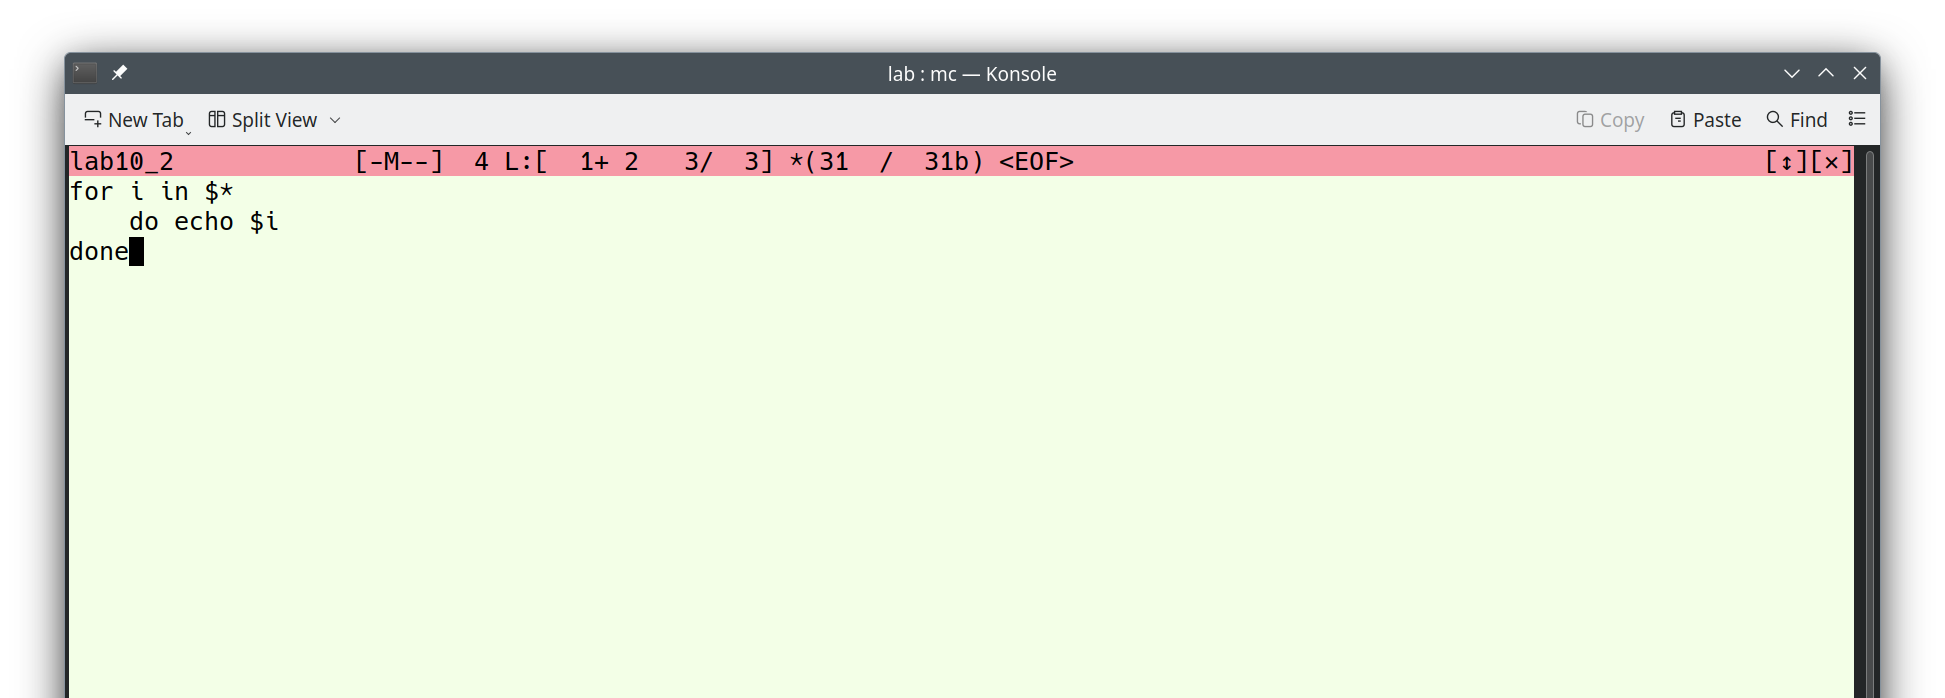
\includegraphics[width=1\textwidth,height=\textheight]{image/4.png}
\caption{код}\label{fig:004}
}
\end{figure}

\begin{figure}
\hypertarget{fig:005}{%
\centering
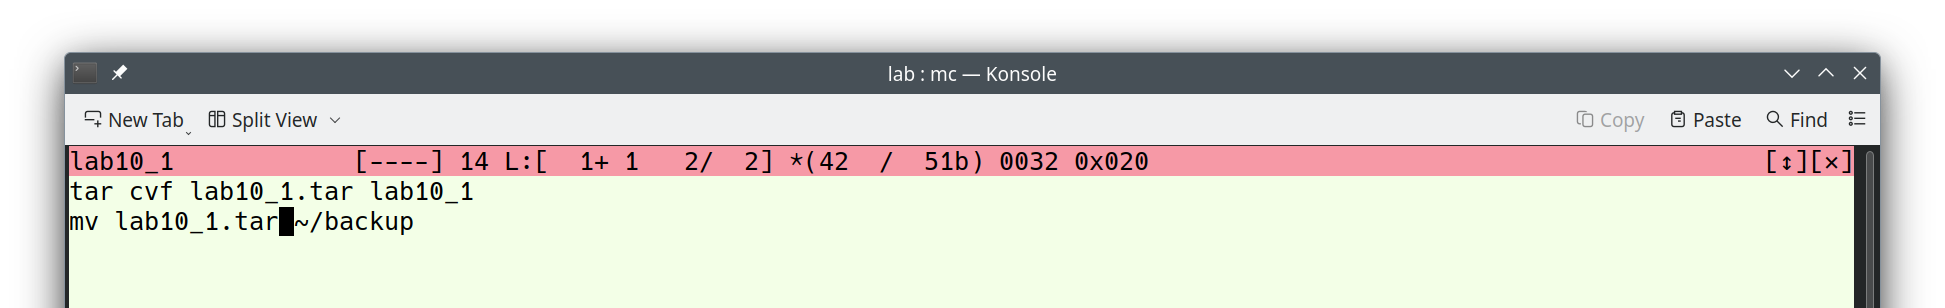
\includegraphics[width=1\textwidth,height=\textheight]{image/1.png}
\caption{результат вывода 11 аргументов}\label{fig:005}
}
\end{figure}

\begin{enumerate}
\def\labelenumi{\arabic{enumi}.}
\setcounter{enumi}{2}
\tightlist
\item
  Пишем скрипт, являющийся аналогом команды ls
\end{enumerate}

\begin{figure}
\hypertarget{fig:006}{%
\centering
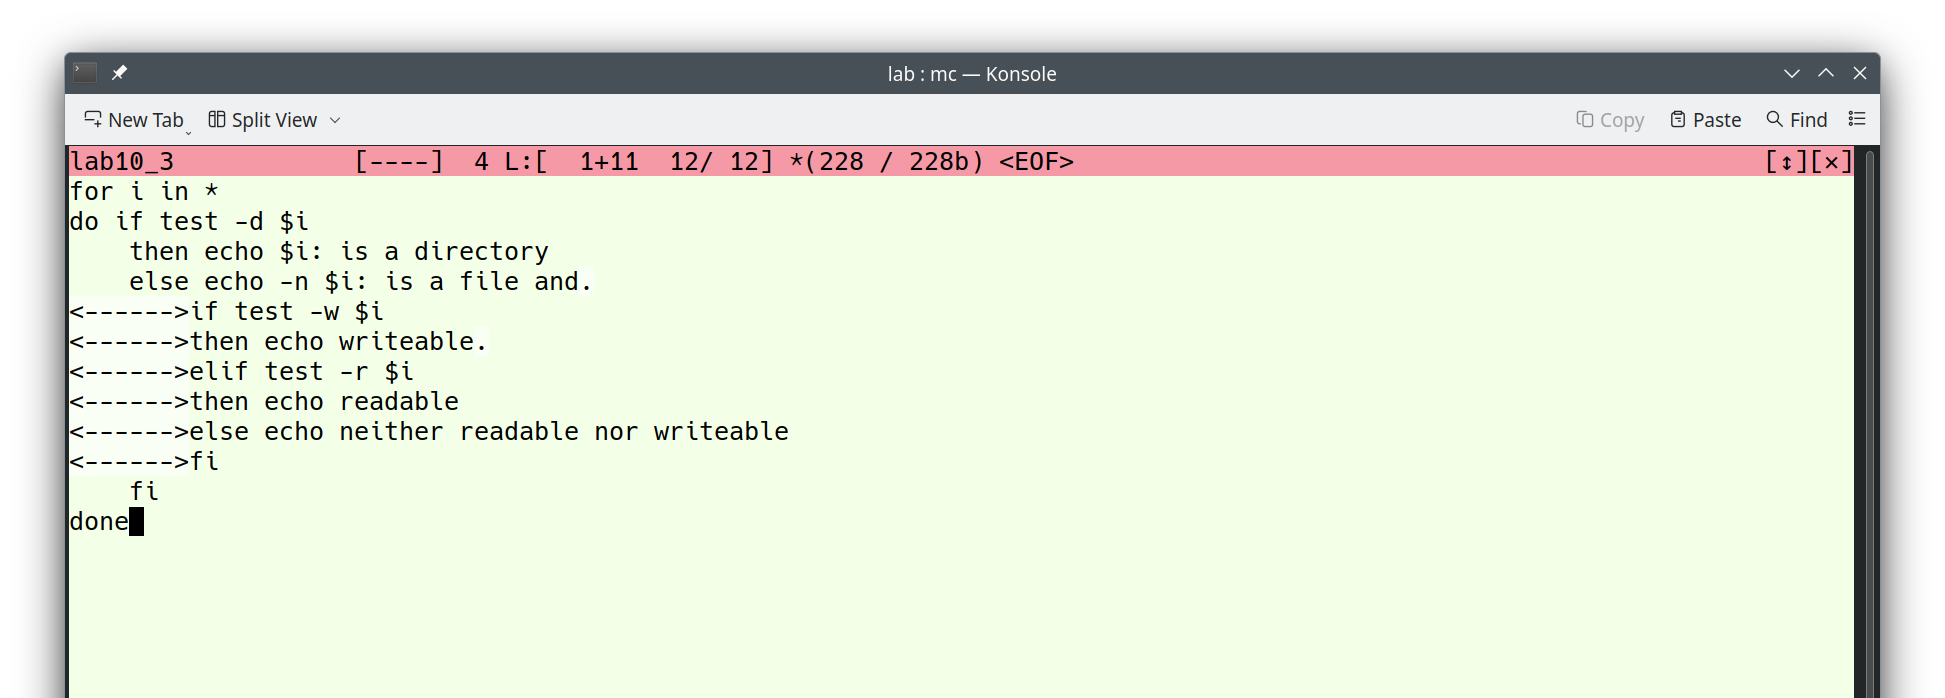
\includegraphics[width=1\textwidth,height=\textheight]{image/6.png}
\caption{код}\label{fig:006}
}
\end{figure}

\begin{figure}
\hypertarget{fig:007}{%
\centering
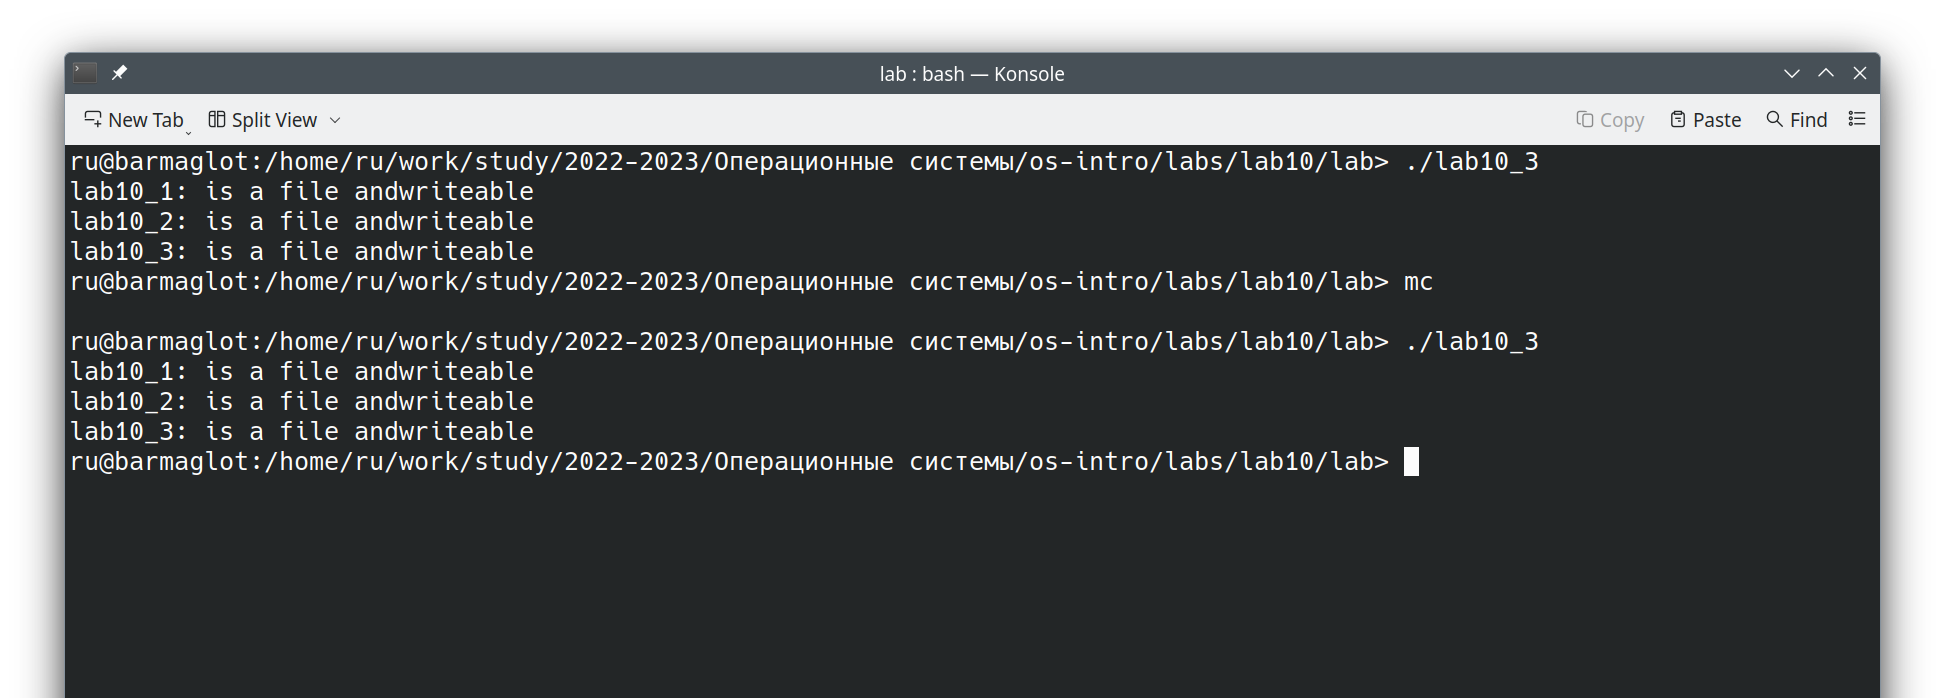
\includegraphics[width=1\textwidth,height=\textheight]{image/7.png}
\caption{вывод информации о файлах}\label{fig:007}
}
\end{figure}

\begin{enumerate}
\def\labelenumi{\arabic{enumi}.}
\setcounter{enumi}{3}
\tightlist
\item
  Пишем скрипт, который вычисляет количество файлов заданного формата в
  указанной директории
\end{enumerate}

\begin{figure}
\hypertarget{fig:008}{%
\centering
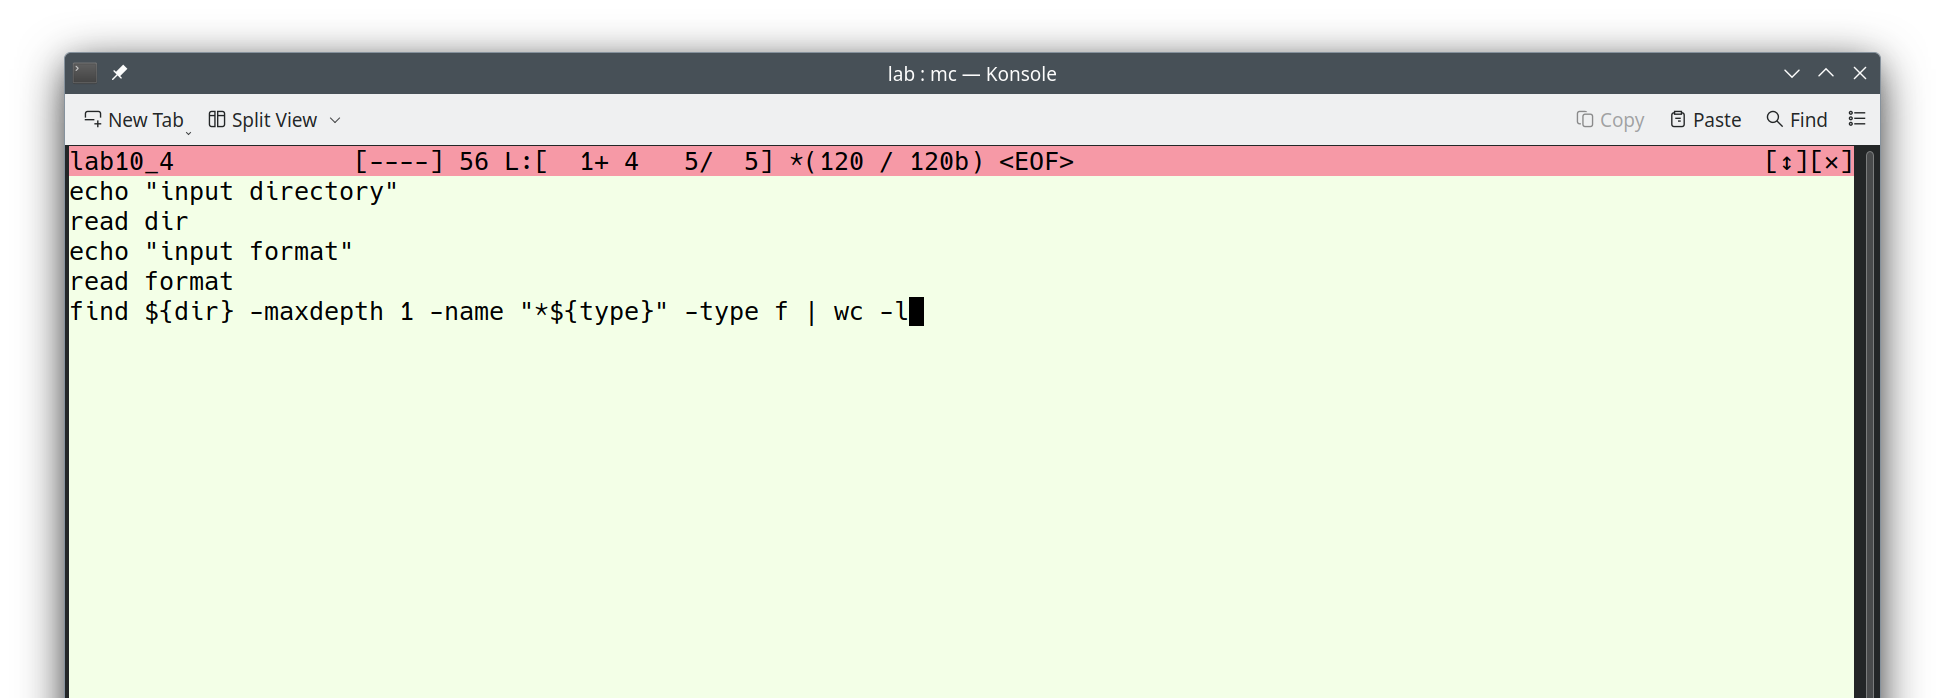
\includegraphics[width=1\textwidth,height=\textheight]{image/9.png}
\caption{код}\label{fig:008}
}
\end{figure}

\begin{figure}
\hypertarget{fig:009}{%
\centering
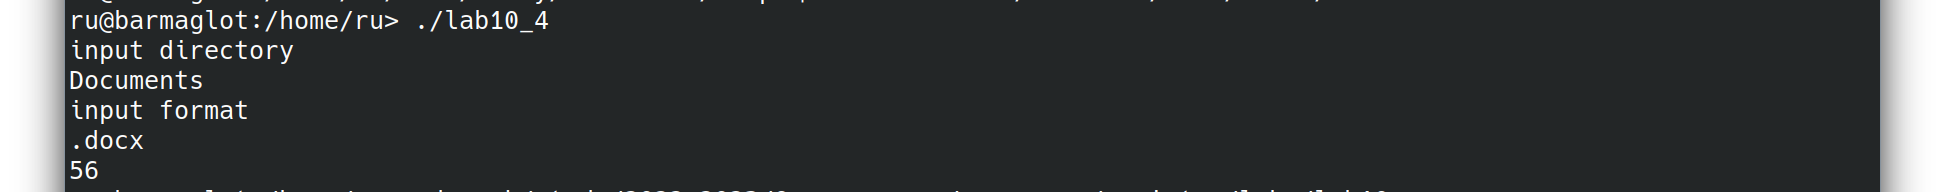
\includegraphics[width=1\textwidth,height=\textheight]{image/8.png}
\caption{вывод информации о каталоге}\label{fig:009}
}
\end{figure}

\hypertarget{ux43eux442ux432ux435ux442ux44b-ux43dux430-ux43aux43eux43dux442ux440ux43eux43bux44cux43dux44bux435-ux432ux43eux43fux440ux43eux441ux44b}{%
\chapter{Ответы на контрольные
вопросы}\label{ux43eux442ux432ux435ux442ux44b-ux43dux430-ux43aux43eux43dux442ux440ux43eux43bux44cux43dux44bux435-ux432ux43eux43fux440ux43eux441ux44b}}

\begin{enumerate}
\def\labelenumi{\arabic{enumi}.}
\tightlist
\item
  Объясните понятие командной оболочки. Приведите примеры командных
  оболочек. Чем они отличаются?
\end{enumerate}

\emph{Командная оболочка} - это программа, позволяющая пользователю
взаимодействовать с операционной системой компьютера. В операционных
системах типа UNIX/Linux наиболее часто используются следующие
реализации командных оболочек: * \emph{оболочка Борна (Bourne shell или
sh)} --- стандартная командная оболочка UNIX/Linux, содержащая базовый,
но при этом полный набор функций; * \emph{С-оболочка (или csh)} ---
надстройка на оболочкой Борна, использующая С-подобный синтаксис команд
с возможностью сохранения истории выполнения команд; * \emph{оболочка
Корна (или ksh)} --- напоминает оболочку С, но операторы управления
программой совместимы с операторами оболочки Борна; * \emph{BASH} ---
сокращение от Bourne Again Shell (опять оболочка Борна), в основе своей
совмещает свойства оболочек С и Корна (разработка компании Free Software
Foundation).

\begin{enumerate}
\def\labelenumi{\arabic{enumi}.}
\setcounter{enumi}{1}
\tightlist
\item
  Что такое POSIX?
\end{enumerate}

\emph{POSIX (Portable Operating System Interface for Computer
Environments)} --- набор стандартов описания интерфейсов взаимодействия
операционной системы и прикладных программ.

\begin{enumerate}
\def\labelenumi{\arabic{enumi}.}
\setcounter{enumi}{2}
\tightlist
\item
  Как определяются переменные и массивы в языке программирования bash?
\end{enumerate}

Команда mark=/usr/andy/bin присваивает значение строки символов
/usr/andy/bin переменной mark типа строка символов, массивы задают
командой set с флагом -А.

\begin{enumerate}
\def\labelenumi{\arabic{enumi}.}
\setcounter{enumi}{3}
\tightlist
\item
  Каково назначение операторов let и read?
\end{enumerate}

Команда let берет два операнда и присваивает их переменной, а команда
read позволяет читать значения переменных со стандартного ввода.

\begin{enumerate}
\def\labelenumi{\arabic{enumi}.}
\setcounter{enumi}{4}
\tightlist
\item
  Какие арифметические операции можно применять в языке программирования
  bash?
\end{enumerate}

C помощью команды let можно производить базовые арифметические операции:
сложение/вычитание, умножение/деление, логические операции.

\begin{enumerate}
\def\labelenumi{\arabic{enumi}.}
\setcounter{enumi}{5}
\tightlist
\item
  Что означает операция (( ))?
\end{enumerate}

В двойные скобки можно записывать выражения для вычисления.

\begin{enumerate}
\def\labelenumi{\arabic{enumi}.}
\setcounter{enumi}{6}
\tightlist
\item
  Какие стандартные имена переменных Вам известны?
\end{enumerate}

PATH, HOME, IFS, MAIL, TERM, LOGNAME. Остальные переменные можно
посмотреть с помощью команды set

\begin{enumerate}
\def\labelenumi{\arabic{enumi}.}
\setcounter{enumi}{7}
\tightlist
\item
  Что такое метасимволы?
\end{enumerate}

Такие символы, как ' \textless{} \textgreater{} * ? \textbar{} ~'' \&,
являются метасимволами и имеют для командного процессора специальный
смысл.

\begin{enumerate}
\def\labelenumi{\arabic{enumi}.}
\setcounter{enumi}{8}
\tightlist
\item
  Как экранировать метасимволы?
\end{enumerate}

Экранирование может быть осуществлено с помощью предшествующего
метасимволу символа , который, в свою очередь, является метасимволом.

\begin{enumerate}
\def\labelenumi{\arabic{enumi}.}
\setcounter{enumi}{9}
\tightlist
\item
  Как создавать и запускать командные файлы?
\end{enumerate}

Создаём файлы командой touch (как и любые другие), запускаем как
исполняемые (с комбинацией ./имя\_файла), предварительно сделав их
исполняемыми

\begin{enumerate}
\def\labelenumi{\arabic{enumi}.}
\setcounter{enumi}{10}
\tightlist
\item
  Как определяются функции в языке программирования bash?
\end{enumerate}

Существует ключевое слово function, после которого следует имя функции и
список команд, заключённых в фигурные скобки. Удалить функцию можно с
помощью команды unset c флагом -f.

\begin{enumerate}
\def\labelenumi{\arabic{enumi}.}
\setcounter{enumi}{11}
\tightlist
\item
  Каким образом можно выяснить, является файл каталогом или обычным
  файлом?
\end{enumerate}

test -d FILE - истина, если FILE является каталогом. test -e FILE -
истина, если FILE является файлом.

\begin{enumerate}
\def\labelenumi{\arabic{enumi}.}
\setcounter{enumi}{12}
\tightlist
\item
  Каково назначение команд set, typeset и unset?
\end{enumerate}

\begin{itemize}
\tightlist
\item
  команда set - вывод списка переменных окружения
\item
  команда unset - удаление переменной из окружения командной оболочки
\end{itemize}

Команда typeset имеет четыре опции для работы с функциями: * -f ---
перечисляет определённые на текущий момент функции; * -ft --- при
последующем вызове функции инициирует её трассировку; * -fx ---
экспортирует все перечисленные функции в любые дочерние программы
оболочек; * -fu --- обозначает указанные функции как автоматически
загружаемые. Автоматически загружаемые функции хранятся в командных
файлах, а при их вызове оболочка просматривает переменную FPATH,
отыскивая файл с одноимёнными именами функций, загружает его и вызывает
эти функции.

\begin{enumerate}
\def\labelenumi{\arabic{enumi}.}
\setcounter{enumi}{13}
\tightlist
\item
  Как передаются параметры в командные файлы?
\end{enumerate}

При вызове командного файла на выполнение параметры ему могут быть
переданы точно таким же образом, как и выполняемой программе. С точки
зрения командного файла эти параметры являются позиционными. Символ \$
является метасимволом командного процессора. Он используется, в
частности, для ссылки на параметры, точнее, для получения их значений в
командном файле. В командный файл можно передать до девяти параметров.
При использовании где-либо в командном файле комбинации символов \$i,
где 0 \textless{} 𝑖 \textless{} 10, вместо неё будет осуществлена
подстановка значения параметра с порядковым номером i, т.е. аргумента
командного файла с порядковым номером i. Использование комбинации
символов \$0 приводит к подстановке вместо неё имени данного командного
файла.

\begin{enumerate}
\def\labelenumi{\arabic{enumi}.}
\setcounter{enumi}{14}
\tightlist
\item
  Назовите специальные переменные языка bash и их назначение
\end{enumerate}

OPTARG и OPTIND. Если ожидается дополнительное значение, то OPTARG
устанавливается в значение этого аргумента (будет равна file\_in.txt для
опции i и file\_out.doc для опции o. OPTIND является числовым индексом
на упомянутый аргумент.

\hypertarget{ux432ux44bux432ux43eux434ux44b}{%
\chapter{Выводы}\label{ux432ux44bux432ux43eux434ux44b}}

Я освоила базовые команды для программирования в оболочке ОС UNIX
